\documentclass[paper]{aiaaNew}

%\usepackage[notref,notcite]{showkeys}


\newenvironment{proof}
{}{}


%\documentstyle[10pt,draft,fancyheadings]{AIAAtran}
%\documentstyle[9pt,twocolumn,technote,twoside]{AIAAtran}


\SubmitName{Schaub}

% for conference paper:

\PaperNumber{xxx}

\CoverFigure{}

\Conference{{\bfseries AIAA Guidance, Navigation and \\ Control 
Conference} \\
            August 10--12,~1998 / Boston, MA}

% for a journal simulation cover page:

\JournalName{Journal of Guidance, Navigation and Control}
\JournalIssue{Volume~xx, Number~xx, Jan.--Feb., 2001, Pages xx--xx}

% journal article simulation:

\ArticleIssue{Vol.~24, No.~1, Jan.--Feb., 2001}% first page
\ArticleHeader{Schaub Et Al: New Penalty Functions}% subsequent pages

% journal note simulation:

\NoteHeader{J.Guidance, Vol.~20, No.~13: Engineering Notes}

% set copyright and other notices to appear
% as a footnote at the bottom of the first page:

%\PaperNotice{\CopyrightB{1998}{Hanspeter Schaub}}

\JournalNotice{Presented as Paper~06--3792 at the AIAA
               Guidance, Navigation and Control Conference, San 
Diego,~CA,
               July~29--31,~1996.
               \CopyrightB{1996}{the authors}}

% load the title, author, and abstract for use with the \maketitle command

\title{Two-Axis Spacecraft Control}
                                
\author{
%
John Clouse%
%
  \thanks{Student,  
  Aerospace Engineering Department.}
  \\
  \emph{\normalsize University of Colorado, Boulder, CO 80309}
}

\abstract{
Underactuation of spacecraft attitude can arise for several reasons.  Whether by design or by fault, many spacecraft must maintain a pointing requirement to complete their missions.  Perfect PD control about two axes is considered to drive a 1-2-1 Euler angle sequence to zero, one axis at a time. Investigated scenarios include elimination of attitude error with and without body rates, as well as inertia tensors that aren't aligned with the body frame. While the controller performed well with a diagonal inertia tensor and starting from rest, complications arose when these conditions weren't met.
}

\usepackage{fixltx2e}
\usepackage{mathtools}
\begin{document}


\maketitle




\section{Introduction}
\PARstart{U}{nderactuated}   
spacecraft attitude scenarios arise when control authority is not available about every body axis.  Such scenarios can happen due to system design, as low cost and hardware simplicity are desirable in spacecraft systems. Propellant or energy saving presents another case, depending on the system design and the mission.  Finally, faulted actuators could require underactuated control to make mission success possible.  
\par
Underactuated control is a well-studied topic.  Coverstone showed how a variable structure controller can detumble a spacecraft with two axes of control\cite{Coverstone96}.  Krishnan et al. considers stabilization of a vehicle with two momentum wheels\cite{Krishnan95}.  Much of the literature focuses on solutions that are not easily implemented during mission operations.  A simpler control design can lead to less-expensive and quicker solutions for craft already in flight.  This paper investigates PD control about two body axes.  Attitude errors are reduced by sequentially driving Euler angles in a 1-2-1 sequence to zero.  

\section{Problem Statement}
This simulation considers the spacecraft's body frame aligned with the principle inertia frame.  Control authority is about the \textit{b}\textsubscript{1} and \textit{b}\textsubscript{2} axes.  An Euler Angle set in the 1-2-1 sequence is being used to drive the attitude error to zero, one axis at a time. Using such a control scheme, the body angular rates are assumed to be about one axis at a time (pure spin about one axis only).  Thus, the general rotational equations of motion\cite{SchaubJunkins}
\[\left [ I \right ]\dot{\boldsymbol{\omega}}=-\left [ \tilde{\boldsymbol{\omega}}\right ]\left [ I \right ]\boldsymbol{\omega}+\mathbf{u}\]
can be simplified: 
\[I_{ii}\ddot{\theta_i}=-(I_{kk}-I_{jj})\omega_j\omega_k+u_i\]
\[\ddot{\theta_i}=\frac{u_i}{I_{ii}}\]

for the controlled axes. The uncontrolled axis has no control authority, so $\dot{\theta}=0$ for \textit{b}\textsubscript{3} .

A controller is chosen such that the equations of motion about the controlled axes resemble a damped harmonic oscillator (a PD controller).  Thus, the controller torque is defined as:
\[u_i=-K_d\dot{\theta_i}+-K_p\theta_i\]
which results in the closed loop dynamics:
\[\ddot{\theta_i}=\frac{-K_d\dot{\theta_i}+-K_p\theta_i}{I_{ii}}\]

\par
The system stability with the controller implemented can be analyzed with Lyapunov stability criteria.  First, a positive definite function is chosen:
\[V= \frac{1}{2}I_{ii} \dot{\theta_i}^2 + \frac{1}{2} K_{pi} \theta_i\]
The time derivative of the positive definite function is then taken.  Appropriate substitutions are then made.
\[\dot{V}=I_{ii}\dot\theta_i\ddot\theta_i+K_{pi}\theta_i\dot\theta_i=\dot\theta_i(I_{ii}\ddot\theta_i+K_p\theta_i)=\dot\theta_i(u_i+K_p\theta_i)\]
\[\dot{V}=-K_{p}\dot\theta_{i}^{2}\]
$\dot{V}$ is globally negative definite. Therefore, with the stated assumptions, this control law is globally stable for pure spins about a body axis.


\section{Controller Design}
The control gains are calculated from the desired parameters $T_s = 70$ seconds and $\zeta=0.98$. For each axis, the relationship of these parameters to the gains Kd and Kp are defined as{\cite{IntroToMech}\cite{NiseControl}}:
\[\zeta=\frac{K_d}{2\sqrt{K_pI}}\]
\[T_s=\frac{-\ln(tolerance\sqrt{1-\zeta^2})}{\zeta\omega_n}\]
where the tolerance is chosen to be 2\% and
\[\omega_n=\sqrt{\frac{K_{p}}{I_{}}}\]

Using a body inertia tensor of
\[I=\begin{bmatrix}
14 & 0 & 0\\ 
0 & 16 & 0\\ 
0 & 0 & 19
\end{bmatrix}\]
the controller gains are found to be
\[\begin{matrix}
K_{p1}=0.0909 & K_{d1}=2.2106 & K_{p2}=0.1038 & K_{d2}=2.5264
\end{matrix}\]
\section{Simulation Design}
The simulator propagates Modified Rodrigues Parameters (MRPs) using 4th-order Runge-Kutta integration. Use of MRPs allows for a compact set, while allowing a switch to the shadow set as the propagated parameters approach a singularity\cite{SchaubJunkins}.  To test the simulation, the rigid body dynamics were propagated for 10 minutes with no control or disturbance torques.  The results can be seen in Figures ~\ref{fig:MRP_Prop} and ~\ref{fig:w_Prop}, which used initial conditions of $\theta_{121}(t_0)=(45^{\circ},60^{\circ},-75^{\circ})^T$, $\boldsymbol{\omega}(t_0)=(1^{\circ}/\textup{s},-2^{\circ}/\textup{s},0.5^{\circ}/\textup{s})^T$, and the previously defined inertia tensor.

 \begin{figure}[htb]
 	\centering
 	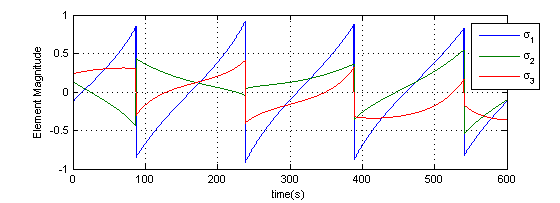
\includegraphics[scale=0.95]{Figures/MRP_Prop}
 	\caption{Propagated MRP attitude.}
 	\label{fig:MRP_Prop}
 \end{figure}
 \begin{figure}[htb]
 	\centering
 	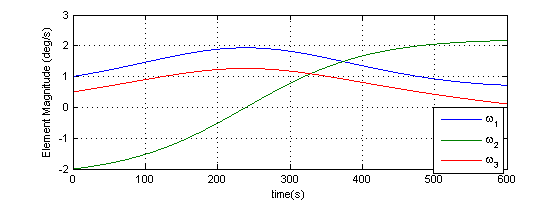
\includegraphics[]{Figures/w_Prop}
 	\caption{Propagated body rates.}
 	\label{fig:w_Prop}
 \end{figure}
Since there are no external torques present, angular momentum is conserved. Kinetic energy in this simulation is also guaranteed to be conserved, due to the assumption of a completely rigid body.  Figures ~\ref{fig:dH} and ~\ref{fig:dT} demonstrate the change in angular momentum and kinetic energy in the simulation, caused by numerical integration error, to be very small.
 \begin{figure}[htb]
 	\centering
 	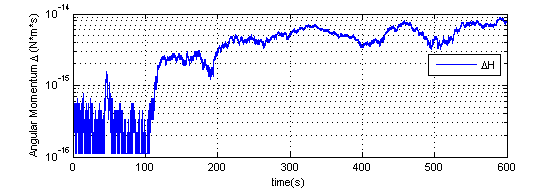
\includegraphics[]{Figures/dH}
 	\caption{Simulation change in angular momentum, no external torques.}
 	\label{fig:dH}
 \end{figure}
 \begin{figure}[htb]
 	\centering
 	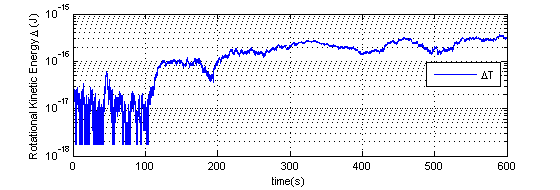
\includegraphics[]{Figures/dT}
 	\caption{Simulation change in kinetic energy, no external torques.}
 	\label{fig:dT}
 \end{figure}

\section{Numerical Simulation: Body at Rest, Principle Inertia Frame Aligned with Body Frame}
The first simulation assumes that the rigid body begins at rest and the body frame is aligned with the principle inertia frame.  Perfect state feedback is fed into the controller.  The initial rotation is chosen to be $\theta_{121}(t_0)=(45^{\circ},60^{\circ},-75^{\circ})^T$.The control strategy is to compute the 1-2-1 Euler angle rotation between the body frame and the reference frame and drive each angle to zero.  Torque will be applied about the $b_1$ axis until $\theta_3=0$, then $b_2$ until $\theta_2=0$, and finally $b_1$ until $\theta_1=0$.  The simulation was written in Matlab.
\par
A geometric singularity is presented when $\theta_2$ approaches zero; in a symmetric Euler sequence, it creates the equivalent of a single axis rotation represented by two elements that can be added together.  The singularity solution is twofold. First, use the atan2 function to avoid division by zero when deriving the sequence from the direction cosine matrix.  Then, when $\theta_2$ is within some small tolerance of zero, $\theta_1$ is set to be the sum of $\theta_1$ and $\theta_3$; $\theta_3$ is set to zero after the summation.  $\theta_1$ is forced to be within $\pm 180^{\circ}$ by adding or subtracting multiples of $360^{\circ}$ as appropriate.
\par
Figures ~\ref{fig:NominalMRP},  ~\ref{fig:NominalRates}, and  ~\ref{fig:NominalU} demonstrate the performance of the controller. The MRPs successfully go to zero with the implemented controller. The body rate and control torque profiles show how the proportional component of the applied torque is dominant when the controller starts to drive each axis.  Eventually the damping component dominates and reduces or eliminates any overshoot.  Tuning was performed to determine when an axis was sufficiently close to zero that the next axis could be controlled with negligible influence from its attitude and rate errors. Too high of a rate error would make the attitude about the previous axis affect the control of the current axis due to the coupling in the equations of motion. Axial states where $\left | \theta_i \right |<10^{-4} $ rad and $\left | \dot{\theta_i} \right |<10^{-5}$ rad had good response time and allowed full control of each axis.
 \begin{figure}[htb]
 	\centering
 	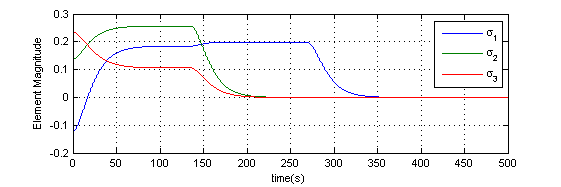
\includegraphics[]{Figures/NominalMRP}
 	\caption{Simulated MRPs.}
 	\label{fig:NominalMRP}
 \end{figure}
 \begin{figure}[htb]
 	\centering
 	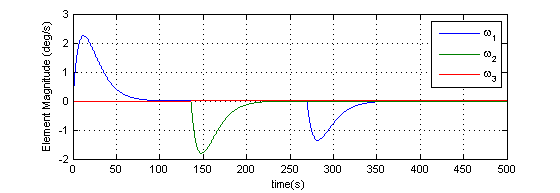
\includegraphics[]{Figures/NominalRates}
 	\caption{Simulated body rates.}
 	\label{fig:NominalRates}
 \end{figure}
 \begin{figure}[htb]
 	\centering
 	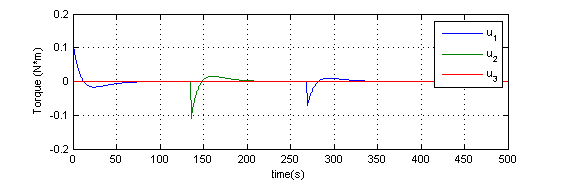
\includegraphics[]{Figures/NominalU}
 	\caption{Simulated control torques.}
 	\label{fig:NominalU}
 \end{figure}
\par

\section{Numerical Simulation: Body Begins with Spin}
The second simulation uses the previous assumptions, but introduces initial body rates. These body rates are pure spins about each axis. An initial rate about the $b_1$ axis was controllable due to that axis being the first to be controlled.  Having an initial rate about the $b_2$ axis did not have the same benefit, due to the gyroscopic effects in the equations of motion. Initial rates about that axis were found to only work with $\left | \omega_2 \right | \leq 10^{-4}$ rad.  Similarly, an initial rate about $b_3$ could only work with $\left | \omega_3 \right | \leq 10^{-5}$ rad.  Tuning the states for which axial control could be performed on the next axis without issue did not yield the ability to control higher initial rates. Instability due to a $10^{-3} $ rad $b_2$ initial rate is shown in figures ~\ref{fig:InitRatesMRP},  ~\ref{fig:InitRatesRates}, and  ~\ref{fig:InitRatesU}.
 \begin{figure}[htb]
 	\centering
 	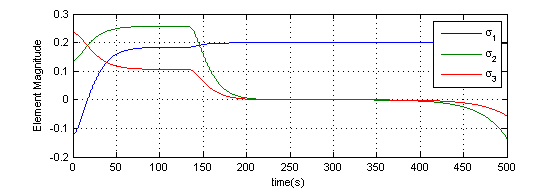
\includegraphics[]{Figures/InitRatesMRP}
 	\caption{Simulated MRPs with initial $b_2$ rate.}
 	\label{fig:InitRatesMRP}
 \end{figure}
 \begin{figure}[htb]
 	\centering
 	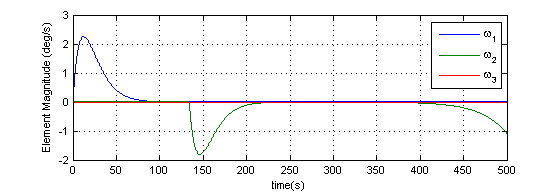
\includegraphics[]{Figures/InitRatesRates}
 	\caption{Simulated body rates with initial $b_2$ rate.}
 	\label{fig:InitRatesRates}
 \end{figure}
 \begin{figure}[htb]
 	\centering
 	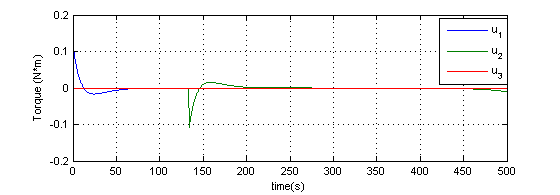
\includegraphics[]{Figures/InitRatesU}
 	\caption{Simulated control torques with initial $b_2$ rate.}
 	\label{fig:InitRatesU}
 \end{figure}
\par
\section{Numerical Simulation: Non-Body-Aligned Principle Inertia Tensor}
The final simulation uses the assumptions of the first, but the principle inertia frame is not aligned with the body frame. An offset from the principle inertia frame to the body frame was defined as the 3-2-1 Euler sequence $[0.5634^{\circ}, 0.6821^{\circ}, 0.4662^{\circ}]$ (magnitude of $1^{\circ}$). The resulting behavior is shown in figures ~\ref{fig:IOffMRP},  ~\ref{fig:IOffRates}, and  ~\ref{fig:IOffU}. Even with a small offset between frames, the system becomes unstable.  The accelerations caused by the cross terms in the inertia tensor cause the attitude error to grow.  This is an untenable situation when controlling about just one axis.
 \begin{figure}[htb]
 	\centering
 	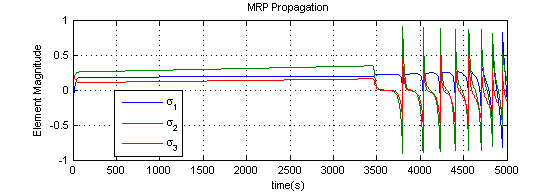
\includegraphics[]{Figures/IOffMRP}
 	\caption{Simulated MRPs with non-aligned principle and body frames.}
 	\label{fig:IOffMRP}
 \end{figure}
 \begin{figure}[htb]
 	\centering
 	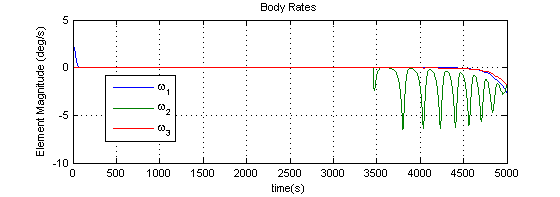
\includegraphics[]{Figures/IOffRates}
 	\caption{Simulated body rates with with non-aligned principle and body frames.}
 	\label{fig:IOffRates}
 \end{figure}
 \begin{figure}[htb]
 	\centering
 	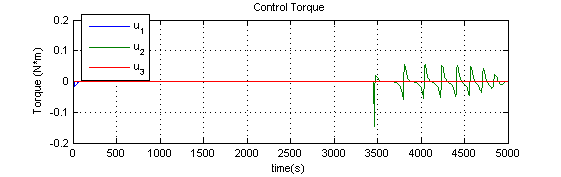
\includegraphics[]{Figures/IOffU}
 	\caption{Simulated control torques with with non-aligned principle and body frames.}
 	\label{fig:IOffU}
 \end{figure}
\par

\section{Conclusion}
Using a PD control law about two axes of a rigid body works well for a body that begins at rest. Almost any amount of spin that is not solely about $b_1$, however, loses its stability guarantee.  Such rates cause accelerations about other axes that compound when trying to drive just one axis.  Due to this, an angular rate regulative controller would be recommended to arrest the rates of a tumbling body before trying to point the vehicle.  
\par
Small rotations between the principle inertia and body frames stops the controller from achieving its goal.  The inertia tensor cross terms cause accelerations about the uncontrolled axes which cause difficulty in controlling one axis at a time.  A solution to this problem would be to guarantee frame alignment, which is especially difficult with any shift in mass.  Another solution would be to gimbal the torque actuators so that they can align with a good estimate of the principle inertia frame. An area ripe for investigation would be to switch between $\theta_2$ and $\theta_3$ to keep $\theta_3$ near-zero.  Even so, it would take a very long time (the first axis took almost an hour to reach "zero-enough") and not be very practical.
\par
Overall, while the controller is asymptotically stable in the originally-assumed situations, it cannot reorient a craft that is tumbling or with torquing actuators that aren't aligned with principle inertia frame axes. These are very real situations that spacecraft will most likely face; the controllers simplicity could thus be an impediment to mission success.  Further work could be done to augment this controller with others, as well as inertia tensor estimates and gimballed actuators.

\bibliographystyle{aiaa}   % Number the references.
\bibliography{ASEN5010ProjectBib}   % Use references.bib to resolve the labels.


\end{document}

